%
% File acl2014.tex
%
% Contact: giovanni.colavizza@epfl.ch
%%
%% Based on the style files for ACL-2013, which were, in turn,
%% Based on the style files for ACL-2012, which were, in turn,
%% based on the style files for ACL-2011, which were, in turn, 
%% based on the style files for ACL-2010, which were, in turn, 
%% based on the style files for ACL-IJCNLP-2009, which were, in turn,
%% based on the style files for EACL-2009 and IJCNLP-2008...

%% Based on the style files for EACL 2006 by 
%%e.agirre@ehu.es or Sergi.Balari@uab.es
%% and that of ACL 08 by Joakim Nivre and Noah Smith

\documentclass[11pt]{article}
\usepackage{acl2014}
\usepackage{times}
\usepackage[hyphens]{url}
\usepackage{latexsym}
\usepackage{graphicx}

\renewcommand{\labelitemi}{$\textendash$}

%\setlength\titlebox{5cm}

% You can expand the titlebox if you need extra space
% to show all the authors. Please do not make the titlebox
% smaller than 5cm (the original size); we will check this
% in the camera-ready version and ask you to change it back.

\title{Explanatory analysis of Amazon reviews}

\author{Fern\'andez David\\
  {\tt david.fernandeznavarro@epfl.ch} \\\And
  Virey Briac\\
  {\tt briac.virey@epfl.ch} \\}

\date{}

\begin{document}
\maketitle
% no longer than 150 words
\begin{abstract}

This report presents the achieved work for the 2017 Applied Data Analysis course at EPFL. The project is based on an Amazon reviews dataset and consists on a detailed explanatory analysis of the data. This document shows the overall process, assumptions and results of such analysis.

The possible influence of other's opinions on one's decision can be taken for granted. The purpose of this research project is to determine whether point of views (such as reviews) can always be relied on.

 
\end{abstract}

\section{Credits}

This project is exclusively based on the {\em Amazon product data} conceived by J. McAuley, UCSD. Instructions and useful advise were given by the Applied Data Analysis (ADA) course instructor, Robert West, EPFL, and the numerous teaching assistants.

\section{Introduction}
The purpose of this report is to analyze the influence of ratings on Amazon.com reviews for all its categories from 1996 to 2014, to check how people rate along time, the relation between price and ratings or category and to see if there is a tendency to rate better those products that usually are more rated. All this knowledge would let us verify some judgments made by the general public including paid critiques on products are not honest, there are more products bought during certain periods so more reviews are done on this time, etc.
This objective will be reached by using Amazon reviews data frame,  Amazon reviews metadata and enriched with small datasets such us the number of births in the United States of America.


\section{Related Work}
The most closely similarly work to ours is the paper where datasets have been taken, written by McAucley J. and Yang A. from  the University of California, San Diego (UCSD) that studies the product-related list that Amazon provides with the customers reviews.

\section{Data Collection}

The {\em Amazon product data} is composed of product reviews along with metadata files for a 142.8-million-reviews collection of Amazon products for a timespan of almost 20 years. The dataset is available through different subsets (raw, per category, metadata, k-scores, rating-only, etc.).

\paragraph{}
{\bf Raw data:} (20 GB compressed) corresponds to the 142.8 million reviews; includes duplicate such as reviews for similar product (DVD and VHS).

{\bf K-scores:} (3.2 GB compressed) duplicates removed; each product and reviewer have at least k-reviews; contains {\em reviewerID}, productID ({\em asin}), rating ({\em overall}), timestamp ({\em reviewTime}).

{\bf Ratings only:} (9.9 GB compressed) duplicates removed; same categories as precedent but no constraint on number of reviews.

{\bf Metadata:} (3.1 GB compressed) includes other informations on product such as {\em price, also\_bought, also\_viewed, brand}, etc.

\paragraph{}
For simplicity reasons, this project was done using {\em ratings only} per category. This enables the exploration of data on a local computer without having to go through the time-consuming process of loading all the data. For some analysis we also need metadata for products for instance, the price of the products.

\section{Data Description}

Considering the 2 tables {\em ratings only} and {\em metadata}, products examined in this project have at least a reviewer, a product ID, a rating and a timestamp (one review per line for each {\em.csv} file), plus a product ID and a price (one product per line).

% Add statistic summary table here

\section{Methodology}
\paragraph{}
Methodology followed could be summarized in just a few steps, facing the problem, studying data, working on data and reaching conclusions.

\paragraph{}
We have started this project by thinking about the general idea, formulating the main questions to be solved before reaching our goals. At the beginning we tried not to be very ambitious because a deeper look to data was still missing. It is also important taking into account that we are a group of only two people, thus the size of the project had to be reduced. With this, and a quick idea of data we have defined some needed fields from the Amazon Reviews.

\paragraph{}
Then, it was the moment for deeper revisions of samples of data, as we have it available in many different formats, we had to choose which one was the most appropriate with us and our way of working. We decided using the {\em.csv} files for ratings, one file per category, that include the {\em reviewerID, rating, asin, timestamp}. In addition, we are going to use some {\em meatadata} files, one per category, mainly for consulting the price of each product.

\paragraph{}
Once we know what data to use, we download and organize it. And then, we do a testing on data, accessing files from the notebook, that the data needed is, in effect, on files and finally that it is easy to use.

\paragraph{}
With the data, we test the accessing and computational speed needed for it. At this moment we decided using our own computers because analysis shows that is feasible.

\paragraph{}
The exploratory analysis allows us to have a deeper understanding of the data, to extract informations from it, which could alter our initial questions. To proceed, the data is organized as much as possible and, memory and CPU efficient methods are considered although this can be a great challenge. 
The main lines of research to explore the data (distribution, from one category to another, absolute or relative, etc.) are based on the reviews, the ratings and the price. Because these attributes are taken individually, they are relatively easy to manipulate.

\paragraph{}
After this investigation process, we decided to modify our initial axis of research and include and temporal scale. This choice was also influenced by the loss of one of our group members on the harsh way to data analysis. Thus, this study is a way to answer the following:

\begin{itemize}
\item {\bf Q1:} How has the amount of reviews changed during time? Is this constant on every category?
\item {\bf Q2:} Is there relation between price of the product and the amount of reviews?
\item {\bf Q3:} Is there relation between category of the product and the amount of reviews?
\item {\bf Q4:} Are the people giving more reviews more satisfied with products?
\end{itemize}

\section{Results}

In the following sections, we present some of the most interesting results, mostly as graphics.

\subsection{Exploratory Analysis}

Through this investigation process, we could derive valuable informations concerning reviews and ratings from the dataset. We also consider a reviews on a varying timescale.

\paragraph{}
First of all, the distribution of reviews per category is shown in the figure \ref{reviews}. The number of reviews with respect to the number of products per category.

\begin{figure}[!h]
\centering
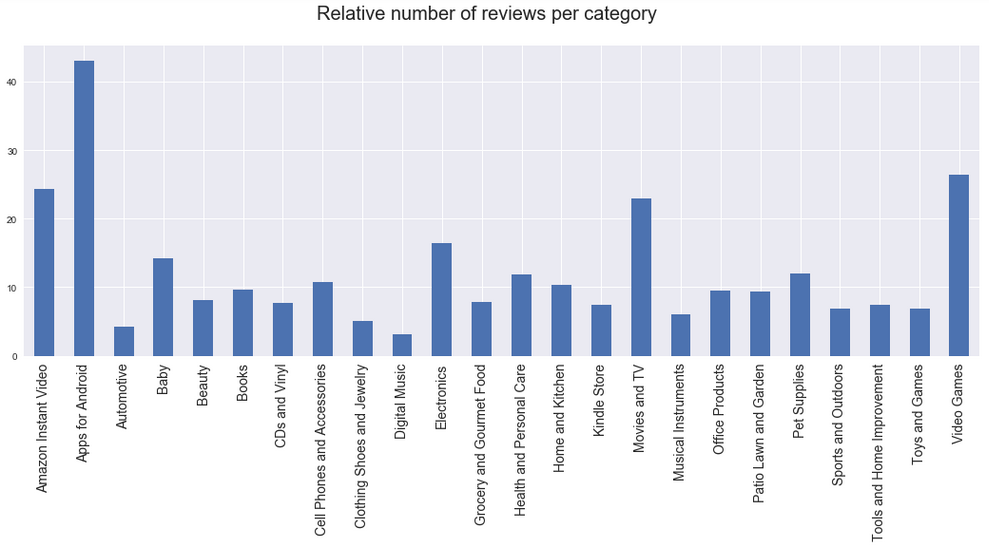
\includegraphics[width=1\linewidth]{reviews.png}
\caption{Number of reviews per category}
\label{reviews}
\end{figure}

The values are, in general, in the same range. Categories with high values correspond to technology-related products. Users may be more familiar with the concept of online reviews.

\paragraph{}
Second part of this analysis focuses on the rating distributions for different categories (figure \ref{ratings}). Once again, these frequency values correspond to a relative frequency with respect to the number of products.

\begin{figure}[!h]
\centering
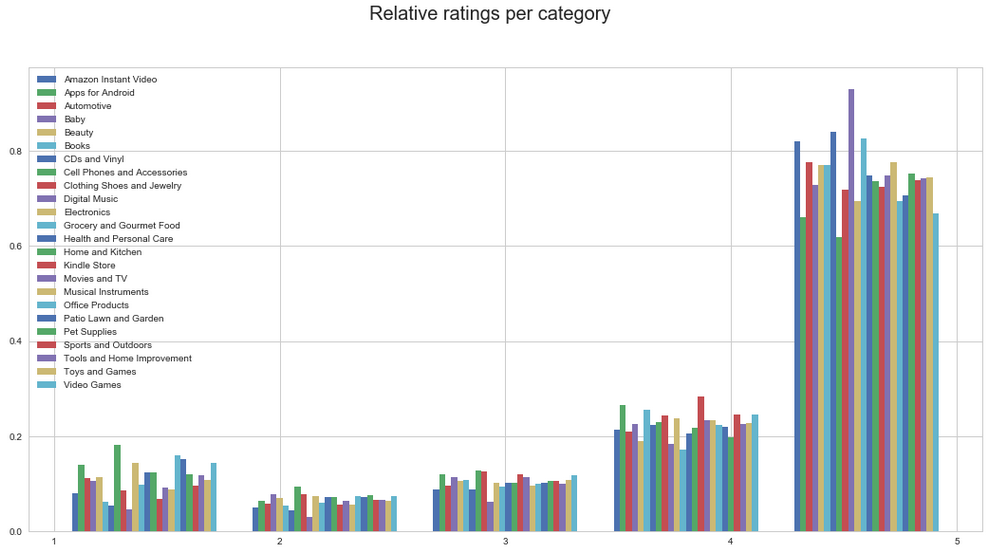
\includegraphics[width=1\linewidth]{ratings.png}
\caption{Number of ratings per category}
\label{ratings}
\end{figure}

The rating distribution hardly depends on the category considered. As we can see, it is heavily skewed. The ratings are mostly {\em 5} and most categories have a minimum on ratings {\em 2}.

\paragraph{}
Finally, we analysed the total number of reviews per year and the results can be seen in the figure {\em\ref{reviews_temp}}. It is clearly visible that the reviews increase with an exponential growth.

\begin{figure}[!h]
\centering
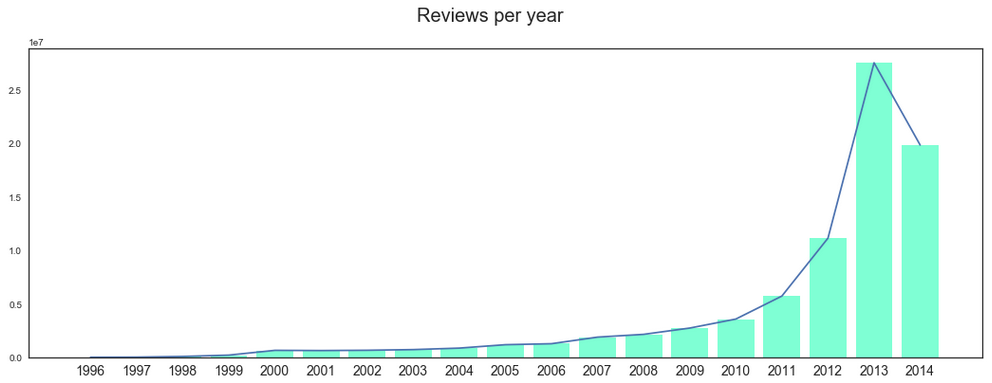
\includegraphics[width=1\linewidth]{reviews_temp.png}
\caption{Number of reviews per year}
\label{reviews_temp}
\end{figure}

The last year (2014) has a lower value as the dataset stops mid-year. To go further, it would be interesting to see how the number of reviews evolves today, if it keeps increasing or if it meets a limit.

\subsection{Q1}

The goal here is to evaluate the evolution of the number of reviews per year. The graph above gave us a first approach but we want to go in-depth. 

\paragraph{}
The figure \ref{q1} corresponds to a more detailed view of these reviews per year. This time, we consider the 24 categories in a log-scale to apprehend the variations at the beginning of the timescale. The small decrease during the last year is still visible here.

\begin{figure}[!h]
\centering
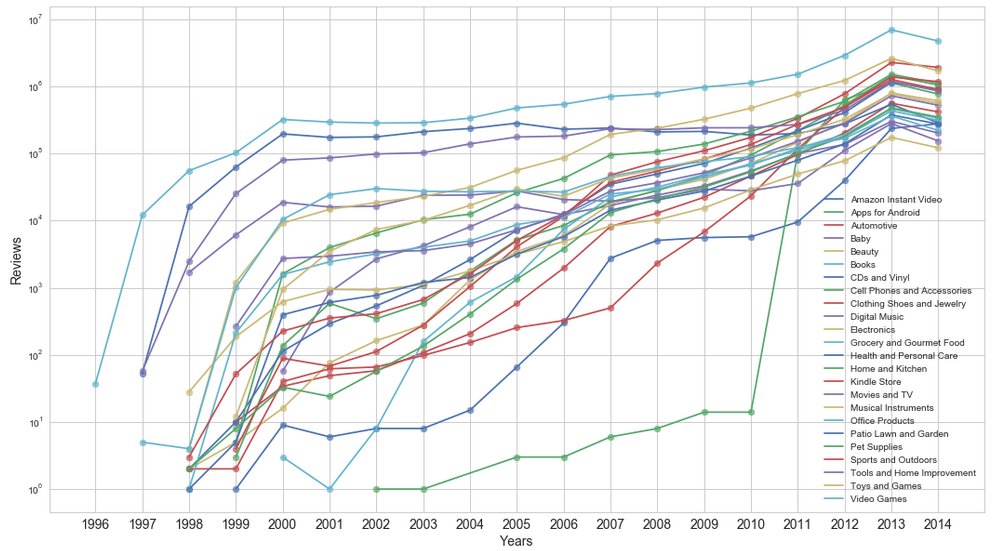
\includegraphics[width=1\linewidth]{q1.png}
\caption{Number of reviews (log-scale) per year}
\label{q1}
\end{figure}

In this figure, we can see how different trends occurred in the early years to merge in one and unique trend. In general, categories related to technology have an odd behaviour. The number of reviews may decrease or suddenly jump from one year to another. This might be associated with the increasing importance of these very same technologies in our lives in the recent years.


\subsection{Q2}
We want to evaluate the relation between price and number of reviews. The following graph (figure \ref{q2c}) shows the scatter plot of each point ({\em price, reviews}) for every categories. The overall trend looks logarithmic. 

\begin{figure}[!h]
\centering
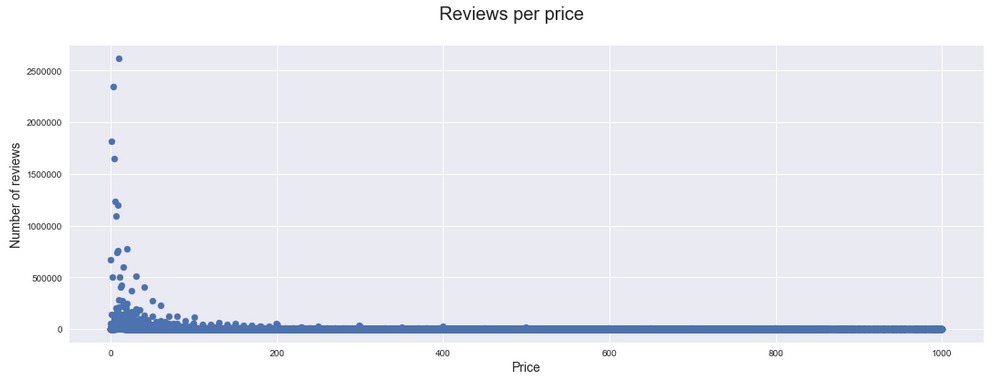
\includegraphics[width=1\linewidth]{q2c.png}
\caption{Reviews per price}
\label{q2c}
\end{figure}

From the distribution of price (graph above), we compute the frequency distribution of price. Each frequency is associated with its number of reviews. In the figure \ref{q2d}, we can see the number of reviews as a function of price for the music industry (3 categories). This scheme can be found in other categories. It was plotted with a log-scale. The smaller the price, the more reviews you have. 

\begin{figure}[!h]
\centering
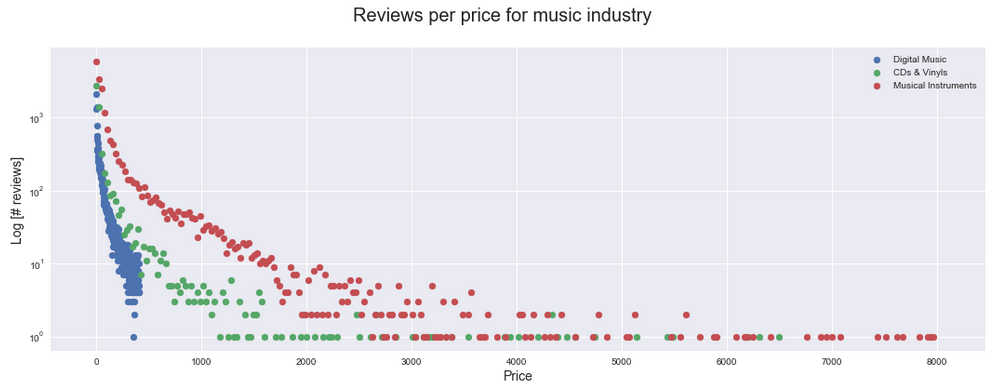
\includegraphics[width=1\linewidth]{q2d.png}
\caption{Products per price {\em Musical Instruments}}
\label{q2d}
\end{figure}

\subsection{Q3}

Once again, we try here to go from the exploratory analysis to a more detailed analysis. For this purpose, we consider the number of reviews per category (figure \ref{q3}). In these boxplots, the median is green, the edges of the box represent the values that respectively 25 and 75\% of the products have and the wiskers to 5 and 95\%. 

\begin{figure}[!h]
\centering
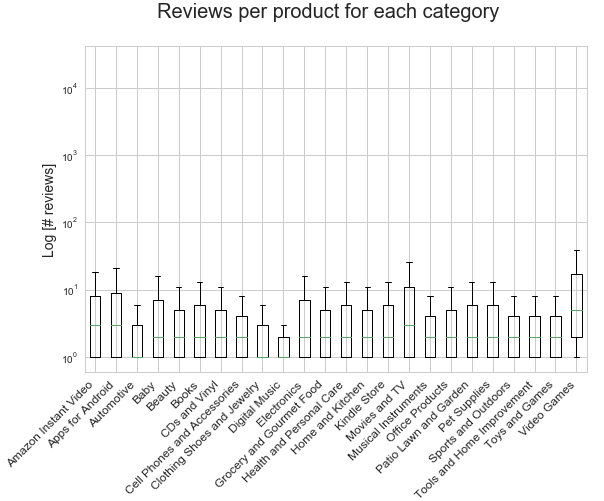
\includegraphics[width=1\linewidth]{q3.png}
\caption{Number of reviews (log-scale)}
\label{q3}
\end{figure}

In this plot, all categories have at least 25\% of the products with at least one review. {\em Video Games} is an exception and has more reviews per product (boxplot shifted upwards). We can see that, once again, technology-related categories ({\em Video Games, Apps for Android, Electronics, Amazon Instant Video, Movies and TV,} etc.) tend to have wider boxplots, and thus products with more reviews. This said, {\em Digital Music} has far too much products for them to be all reviewed and other platforms allow to listen to music for free. 
Unfortunately, the outliers are not visible with too many categories.

\subsection{Q4}

In this part, we want to see whether the top reviewers have a different rating habit compared to the rest of the reviewers. The figure \ref{q4} is clearly showing that, while the top-20 reviewers tend to give less extreme ratings ({\em 1,2} and {\em 5}), they use more frequently the average grades such as {\em 3} and {\em 4}.

\begin{figure}[!h]
\centering
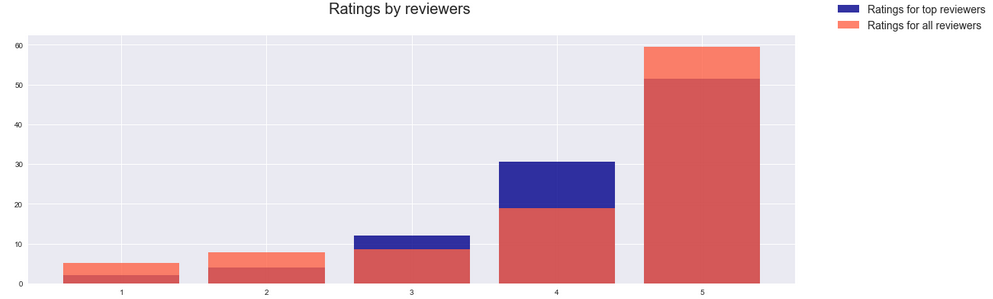
\includegraphics[width=1\linewidth]{q4.png}
\caption{Ratings by (top-)reviewers}
\label{q4}
\end{figure}

It would be possible to go further into the analysis by, for example, determining in which categories these top reviewers grade mostly, or consider more than 2 types of reviewers.

\section{Conclusion}

Working on this project has been a good training for our data scientific life, we have learned the basics, faced a data problem, and dealt with large datasets.

We have proven that both the number of reviews and the number of products reviewed are constantly increasing so that reviews are a key factor for Amazon.

Something we have also learned is that people tend to review (and thus to buy) more cheap products than expensive one in each category.

From question three, we could say that even though the number of reviews per product is similar between categories, there are some that out stands from the others (in particular for technology-related products).

And about satisfaction, we can definitely say that yes, those with more reviews tend to rate better, the rarely use low scores.

Handling the data, we have learned many methods that use less time and memory and so are more efficient. This can be seen along the code, with important improvements on data structures. Also that the drop of a member was a difficulty but we knew how to face it!

Finally, is this useful for social good? Definitely yes! It`s clear that reviews are helpful and take part in their purchase decisions, but they are not only done because of the motivation of knowing that you are helping someone, but also because of money and free products sometimes, so take care about what you buy and don't be influenced only by one opinion but by a mix of them, taking into account the pros and cons of products.

% I don't know why, the references are not ordered as they should

\begin{thebibliography}{}

\bibitem[\protect\citename{chen}2017]{Chen:17}
Chen Y.
\newblock 2017.
\newblock {\em Confessions of a paid Amazon review writer} [online].
\newblock Digiday
\newblock \url{https://digiday.com/marketing/vendors-ask-go-around-policy-confessions-top-ranked-amazon-review-writer/} [Accessed 8 Dec. 2017].

\bibitem[\protect\citename{data}2017]{Data:17}
Data.un.org.
\newblock 2017.
\newblock {\em UNdata | record view | Live births by month of birth} [online].
\newblock \url{http://data.un.org/Data.aspx?d=POP&f=tableCode%3A55} [Accessed 14 Dec. 2017].

\bibitem[\protect\citename{hall}2017]{Hall:17}
Hall M.
\newblock 2017.
\newblock {\em Amazon.com | History \& Facts} [online].
\newblock Encyclopedia Britannica
\newblock \url{https://www.britannica.com/topic/Amazoncom} [Accessed 11 Dec. 2017].

\bibitem[\protect\citename{he}2016]{He:16}
He R. and McAuley J.
\newblock 2016.
\newblock {\em Modeling the visual evolution of fashion trends with one-class collaborative filtering}.
\newblock WWW.

\bibitem[\protect\citename{mcauley}2015]{McAuley:15}
McAuley J.; Targett C.; Shi J. and van den Hengel  A.
\newblock 2015.
\newblock {\em Image-based recommendations on styles and substitutes}.
\newblock SIGIR.

\bibitem[\protect\citename{quinn}2015]{quinn:15}
Quinn J.
\newblock 2015.
\newblock {\em Amazon timeline: from internet bookshop to the world's biggest online retailer} [online].
\newblock Telegraph
\newblock \url{http://www.telegraph.co.uk/technology/amazon/11801515/Amazon-timeline-from-internet-bookshop-to-the-worlds-biggest-online-retailer.html} [Accessed 5 Dec. 2017].


\bibitem[\protect\citename{dlab}2017]{dlab:17}
West Robert.
\newblock 2017.
\newblock {\em Applied Data Analysis (ADA)} [online].
\newblock \url{https://dlab.epfl.ch/teaching/fall2017/cs401/} [Accessed 14 Dec. 2017].

\end{thebibliography}

\end{document}
